\section{Preliminary experiments and FGLM}
\label{sec:fglm}

%{\it Gr\"obner basis Complexity:} To compute a Gr\"obner basis for
%$J + J_0$ over $\Fq$, the following result is known \cite{gao:gf-gb-ms}:  

\begin{Theorem}
(From \cite{lv:date2012}:) Let $J + J_0 = \langle f_1, \dots, f_s, ~x_1^q -
  x_1, \dots, x_d^q - x_d\rangle \subset \Fq [x_1, \dots, x_d]$ be an
  ideal. The time and space complexity of Buchberger's algorithm to
  compute a Gr\"obner basis of $J + J_0$ is bounded by $q^{O(d)}$.
 assuming that the length of input $f_1, \dots, f_s$ is dominated by
 $q^{O(d)}$.  
\end{Theorem}

In our case $q = 2^k$, and when $k$ and $d$ are large, this complexity 
makes verification infeasible. The impact of this complexity is clearly
visible in the results of preliminary experiments (TABLE \ref{tab:sT}).
The experiments are conducted with Mastrovito \cite{mastro:1989}
multiplier circuits of various word sizes $k$. Each multiplier
computes the polynomial function  $Y = \F(A,B) = A \cdot B$ over
$\Fkk$, where $Y, A, B$ are $k$-bit vectors. We extract the 
Boolean gate-level operators $J$ and generate vanishing polynomials $J_0$.
Then we compute the Gr\"obner basis of $J + J_0$
with respect to abstraction term order $>$. The computation was performed
using the "slimgb" command in the {\sc Singular'} computer algebra
tool \cite{DGPS}. The resulting Gr\"obner bases contained a polynomial
$Y + A \times B$.  
These experiments were run on a 64-bit Ubuntu OS running on a 2.4GHz 
Intel QuadCore processor with 8Gb of memory. The approach is
infeasible beyond 40-bit datapath size, as the Gr\"obner basis engine
encounters a memory explosion. BDDs cannot be constructed for
any of these circuits. 

%In Elliptic Curve Cryptography, the 
%minimum suggested word-size is 163 bits, as set by the US National Institute 
%for Standards and Technology. Therefore, I wish to conduct research to make 
%this approach scalable.

\begin{table}[h]
{\small
	\begin{center}
	    \caption{Gr\"obner Basis runtime for
              Mastrovito Multipliers in Singular using Abstraction
              Term Order $>$.}\label{tab:sT} 
	    \begin{tabular}{|c|c||c|} 
	        \hline
		Word Size ($k$) & \# Polynomials (\# gates) & Time (minutes)   \\
		\hline
	        $16$	&  $1,871$  & $2.4$ \\
		$24$	&  $3,135$  & $12$  \\
	        $32$	&  $5,549$  & $22.6$ \\
	        $40$	&  $8,587$  & $266$ \\
		$48$	& $12,327$  & NA (Out of Memory) \\
	        \hline
	    \end{tabular}
	\end{center} 
}
\end{table}

{\it Proposed FGLM Approach:} To make this approach scalable, we are
investigating the use of the FGLM algorithm \cite{fglm}. This
algorithm provides a method for converting a Gr\"obner basis in one
term ordering to a  Gr\"obner Basis in another term ordering.
We use this method in conjunction with following result which was
derived and proved in \cite{lv:date2012}: 

\begin{Theorem} \label{thm:top-order}
Let $C$ be any arbitrary combinational circuit. Let $\{x_1, \dots,
x_d\}$ denote the set of all variables (signals) in the circuit,
i.e. the primary input, intermediate and primary output
variables. Perform a {\it reverse topological traversal} of the
circuit and order the variables such that $x_i > x_j$ if $x_i$ appears
earlier in the reverse topological order. Impose a lex term order to
represent each gate as a polynomial $f_i$,
s.t. $f_i = x_i + \text{tail}(f_i)$. Then the set of all polynomials 
$G_1 = \{f_1, \dots, f_s, x_i^q - x_i: i = 1, \dots, d\}$ constitutes
a Gr\"obner basis.
%, as $lt(f_i)$ and $ lt(f_j)$ for $i\neq j$ are relatively prime.
\end{Theorem}



Using the term ordering specified by \cite{lv:date2012}, which we
denote $>_1$,  we can obviate the need to compute a Gr\"obner
basis. Imposing the monomial ordering $>_1$ already makes $G_1$ a
Gr\"obner basis of $J + J_0$. Now we apply the FGLM algorithm to
transform the Gr\"obner basis into another basis w.r.t. the
abstraction ordering $>$.  This new basis will also definitely contain
a polynomial in the form of $Y + \F(A)$ as desired. By using FGLM to
convert the Gr\"obner basis from $>_1$ to $>$, we are hoping to avoid
the complexity presented by computing a Gr\"obner basis over the
abstraction ordering $>$.  


\begin{Example}
\label{ex:myapproach}
{\it
Let us revisit the 2-bit multiplier circuit from Example \ref{ex:twomult}, 
shown in Fig. \ref{fig:mul2bit}. 
 
%\begin{figure}[htb]
%\centerline{
%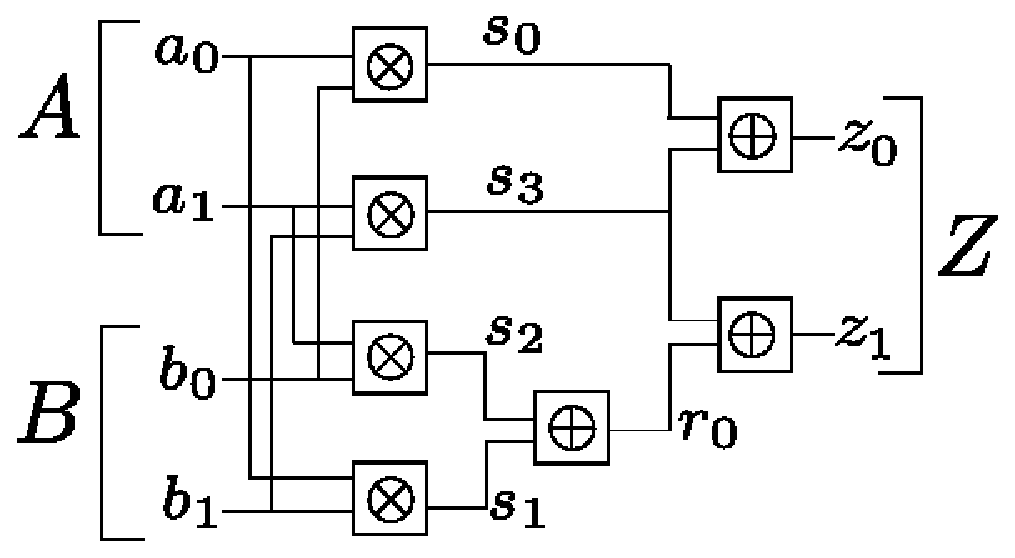
\includegraphics[scale=0.35]{2bitmult.eps}
%}
%\caption{\small A 2-bit Multiplier over ${\mathbb{F}}_{2^2}$. The gate
%  $\otimes$ corresponds to AND-gate, i.e. bit-level multiplication
%  modulo 2. The gate $\oplus$ corresponds to XOR-gate, i.e. addition
%  modulo 2.} 
%\label{fig:mul2bit2}
%\end{figure}
As before, we can describe the functionality of this circuit, $J$, using the
following polynomials: $f_1: Z+z_0+z_1\alpha; ~~f_2: B+b_0+b_1\alpha; ~~f_3: A+a_0+a_1 \alpha
; ~~f_4: s_0+a_0 \cdot b_0; ~~f_5: s_1+a_0 \cdot b_1; ~~f_6:
s_2+a_1 \cdot b_0; ~~f_7: s_3+a_1 \cdot b_1; ~~f_8: r_0+s_1 + s_2;
~~f_9: z_0+s_0 + s_3; ~~f_{10}: z_1 + r_0 + s_3$.
By imposing the monomial order $>_1$, $J+J_0$ is already a Gr\"obner basis, 
where $J_0$ is the ideal of vanishing polynomials of the circuit:
$~~f_{11}: a_0^2+a_0; ~~f_{12}: a_1^2+a_1; ~~f_{13}: b_0^2+b_0;
~~f_{14}: b_1^2+b_1; ~~f_{15}: s_0^2+s_0; ~~f_{16}: s_1^2+s_1;
~~f_{17}: s_2^2+s_2; ~~f_{18}: s_3^2+s_3; ~~f_{19}: r_0^2+r_0;
~~f_{20}: z_0^2+z_0; ~~f_{21}: z_1^2+z_1$. We denote this Gr\"obner
basis as $G_1 = \{f_1, \dots, f_{21}\}$. Using the FGLM algorithm 
("fglm" command in  Singular) we convert $G_1$
from ordering $>_1$ to $G$ with the abstraction term ordering $>$. 
The resulting Gr\"obner basis $G$ contains the 
polynomial $Z \cdot (\alpha+1)+A \cdot B \cdot (\alpha+1)$, 
which can be equivalently reduced to $Z+A \cdot B$.
}
\end{Example}

FGLM exploits concepts from algebraic geometry and sparse linear
algebra to transform the Gr\"obner basis. While a detailed exposition
of FGLM is beyond the scope of this paper, we demonstrate its
operation on the 2-bit multiplier shown in Example
\ref{ex:myapproach}.  

\begin{Example}
\label{ex:approach}
{\it
FGLM begins by taking the least variable in the the abstraction term 
ordering, ($A$ in our case). Starting with $m=0$, it computes $A^m
\xrightarrow{G_1}_+r$. It checks whether the remainder $r$ can be
represented as a linear combination of any remainders calculated thus
far. If so, it adds this  representation to $G$ and moves on to the
next monomial; otherwise it  increments $m$ and repeats $A^m
\xrightarrow{G_1}_+r$ computation. 

\begin{itemize}
\item $A^0 \xrightarrow{G_1}_+ 1$
\item $A^1 \xrightarrow{G_1}_+ a_0+ a_1 \alpha$
\item $A^2 \xrightarrow{G_1}_+ a_0+a_1 \cdot (\alpha+1) $
\item $A^3 \xrightarrow{G_1}_+ a_0 \cdot a_1+a_0+a_1$
\item $A^4 \xrightarrow{G_1}_+ a_0+ a_1 \alpha = A$
\end{itemize}

$A^4$ can be composed of $A$, so $A^4 - A$ is added to $G$. Similarly,
$B^4 - B$ is also added to $G$. Continue to the next variable $Z$ in
the order as we have ``circuit variables'' $> Z > A > B$. 
\begin{itemize}
\item $Z^1 \xrightarrow{G_1}_+ a_0 \cdot b_0+(\alpha) \cdot a_0 \cdot
  b_1+(\alpha) \cdot a_1 \cdot b_0+(\alpha^2) \cdot a_1 \cdot b_1 = 
a_0(b_0 + b_1 \alpha) + a_1\alpha (b_0 + b_1 \alpha) = (a_0 + a_1
\alpha)(b_0 + b_1 \alpha) = A   \cdot B$ 
\end{itemize}
$Z$ is found to be a function of $A$ and $B$, therefore $Z - AB$ is
added to $G$.
}
\end{Example}

FGLM continues to convert the rest of the monomials into the new ordering. However, 
since we are only looking for $Y=\F(A)$ polynomial representation, we
can make this approach even more efficient by restricting the
conversion to only the word-level variables of the circuit. This idea
is currently under development. 

\section{Conclusions}
\label{sec:concl}

This paper has described an approach to derive a word-level, canonical
polynomial representation from combinational circuits using Gr\"obner
bases. Our approach interprets the function of the circuit $f: \B^k
\rightarrow \B^k$ as a polynomial function over Galois fields $f: \Fkk
\rightarrow \Fkk$. By deriving a set of polynomials corresponding to
the circuit (ideal $J + J_0$), and computing its Gr\"obner basis
w.r.t. a specific elimination (abstraction) term order, the canonical
representation of this circuit can be derived. As Gr\"obner basis
computation exhibits high complexity, we are currently investigating
the use of the FGLM algorithm to make our approach scalable. 
